%
% ---------------------------------------------------------------
% Copyright (C) 2012-2018 Gang Li
% ---------------------------------------------------------------
%
% This work is the default powerdot-tuliplab style test file and may be
% distributed and/or modified under the conditions of the LaTeX Project Public
% License, either version 1.3 of this license or (at your option) any later
% version. The latest version of this license is in
% http://www.latex-project.org/lppl.txt and version 1.3 or later is part of all
% distributions of LaTeX version 2003/12/01 or later.
%
% This work has the LPPL maintenance status "maintained".
%
% This Current Maintainer of this work is Gang Li.
%
%

\documentclass[
 size=14pt,
 paper=smartboard,  %a4paper, smartboard, screen
 mode=present, 		%present, handout, print
 display=slides, 	% slidesnotes, notes, slides
 style=tuliplab,  	% TULIP Lab style
 pauseslide,
 fleqn,leqno]{powerdot}


%我自己增加的两端对其用
\usepackage{ragged2e}
\renewcommand{\raggedright}{\leftskip=0pt \rightskip=0pt plus 0cm}


\usepackage{cancel}
\usepackage{caption}
\usepackage{stackengine}
\usepackage{smartdiagram}
\usepackage{attrib}
\usepackage{amssymb}
\usepackage{amsmath} 
\usepackage{amsthm} 
\usepackage{mathtools}
\usepackage{rotating}
\usepackage{graphicx}
\usepackage{boxedminipage}
\usepackage{rotate}
\usepackage{calc}
\usepackage[absolute]{textpos}
\usepackage{psfrag,overpic}
\usepackage{fouriernc}
\usepackage{pstricks,pst-3d,pst-grad,pstricks-add,pst-text,pst-node,pst-tree}
\usepackage{moreverb,epsfig,subfigure}
\usepackage{color}
\usepackage{booktabs}
\usepackage{etex}
\usepackage{breqn}
\usepackage{multirow}
\usepackage{natbib}
\usepackage{bibentry}
\usepackage{gitinfo2}
\usepackage{siunitx}
\usepackage{nicefrac}
%\usepackage{geometry}
%\geometry{verbose,letterpaper}
\usepackage{media9}
\usepackage{animate}
%\usepackage{movie15}
\usepackage{auto-pst-pdf}

%\usepackage{breakurl}
\usepackage{fontawesome}
\usepackage{xcolor}
\usepackage{multicol}



\usepackage{verbatim}
\usepackage[utf8]{inputenc}
\usepackage{dtk-logos}
\usepackage{tikz}
\usepackage{adigraph}
%\usepackage{tkz-graph}
\usepackage{hyperref}
%\usepackage{ulem}
\usepackage{pgfplots}
\usepackage{verbatim}
\usepackage{fontawesome}


\usepackage{todonotes}
% \usepackage{pst-rel-points}
\usepackage{animate}
\usepackage{fontawesome}

\usepackage{listings}
\lstset{frameround=fttt,
frame=trBL,
stringstyle=\ttfamily,
backgroundcolor=\color{yellow!20},
basicstyle=\footnotesize\ttfamily}
\lstnewenvironment{code}{
\lstset{frame=single,escapeinside=`',
backgroundcolor=\color{yellow!20},
basicstyle=\footnotesize\ttfamily}
}{}


\usepackage{hyperref}
\hypersetup{ % TODO: PDF meta Data
  pdftitle={Kaggle Bike-sharing-demand sildes},
  pdfauthor={Bing Liu},
  pdfpagemode={FullScreen},
  pdfborder={0 0 0}
}


% \usepackage{auto-pst-pdf}
% package to show source code

\definecolor{LightGray}{rgb}{0.9,0.9,0.9}
\newlength{\pixel}\setlength\pixel{0.000714285714\slidewidth}
\setlength{\TPHorizModule}{\slidewidth}
\setlength{\TPVertModule}{\slideheight}
\newcommand\highlight[1]{\fbox{#1}}
\newcommand\icite[1]{{\footnotesize [#1]}}

\newcommand\twotonebox[2]{\fcolorbox{pdcolor2}{pdcolor2}
{#1\vphantom{#2}}\fcolorbox{pdcolor2}{white}{#2\vphantom{#1}}}
\newcommand\twotoneboxo[2]{\fcolorbox{pdcolor2}{pdcolor2}
{#1}\fcolorbox{pdcolor2}{white}{#2}}
\newcommand\vpspace[1]{\vphantom{\vspace{#1}}}
\newcommand\hpspace[1]{\hphantom{\hspace{#1}}}
\newcommand\COMMENT[1]{}

\newcommand\placepos[3]{\hbox to\z@{\kern#1
        \raisebox{-#2}[\z@][\z@]{#3}\hss}\ignorespaces}

\renewcommand{\baselinestretch}{1.2}


\newcommand{\draftnote}[3]{
	\todo[author=#2,color=#1!30,size=\footnotesize]{\textsf{#3}}	}
% TODO: add yourself here:
%
\newcommand{\gangli}[1]{\draftnote{blue}{GLi:}{#1}}
\newcommand{\shaoni}[1]{\draftnote{green}{sn:}{#1}}
\newcommand{\gliMarker}
	{\todo[author=GLi,size=\tiny,inline,color=blue!40]
	{Gang Li has worked up to here.}}
\newcommand{\snMarker}
	{\todo[author=Sn,size=\tiny,inline,color=green!40]
	{Shaoni has worked up to here.}}

%%%%%%%%%%%%%%%%%%%%%%%%%%%%%%%%%%%%%%%%%%%%%%%%%%%%%%%%%%%%%%%%%%%%%%%%
% title
% TODO: Customize to your Own Title, Name, Address
%
\title{what's cooking}
\author{
Bing Liu
\\
\\Jilin University
\\College of Computer Science and Technology
}
\date{\gitCommitterDate}
%\date{\today} %暂时手写改动

% Customize the setting of slides
\pdsetup{
% TODO: Customize the left footer, and right footer
rf=\href{http://www.tulip.org.au}{
Last Changed by: \textsc{\gitCommitterName}\ \gitVtagn-\gitAbbrevHash\ (\gitAuthorDate)
%Last Changed by: \textsc{Bing Liu}\ \gitVtagn-\gitAbbrevHash\ (\today)
},
cf={Flip01-Kaggle-Presentation},
}


\begin{document}

\maketitle

%\begin{slide}{Overview}
%\tableofcontents[content=sections]
%\end{slide}


%%==========================================================================================
%%
\begin{slide}[toc=,bm=]{Table Of Content}
\tableofcontents[content=currentsection,type=1]
\end{slide}
%%
%%==========================================================================================


\section{Overview}

%%==========================================================================================
%%
\begin{slide}{Description and Evaluation}

\begin{itemize}
\item \textbf{Description}

\medskip    %\smallskip \medskip
In this competition, participants are asked to predict the category of a dish's cuisine given a list of its ingredients. 

\bigskip
\bigskip
\item \textbf{Evaluation}

\medskip
Submissions are evaluated on the categorization accuracy (the percent of dishes that you correctly classify).

\end{itemize}

\end{slide}
%%
%%==========================================================================================

%%==========================================================================================
%%
%\begin{slide}{Data}
%\raggedright
%\end{slide}
%%
%%==========================================================================================



\section{Data}

%%==========================================================================================
%%
\begin{slide}{Data Description and Explorer}

\begin{itemize}
	\item \textbf{Data Description}
	
	\medskip
	In the dataset, it include the recipe id, the type of cuisine, and the list of ingredients of each recipe (of variable length). The data is stored in JSON format.\\
	
	In the test file test.json, the format of a recipe is the same as train.json, only the cuisine type is removed, as it is the target variable you are going to predict.
	\bigskip
	\item \textbf{Data Explorer}
	
	\begin{itemize}
		\smallskip
		\item \textbf{train.json} -- the training set containing recipes id, type of cuisine, and list of ingredients. It contains 39774 entries.
		\smallskip
		\item \textbf{test.json} -- the test set containing recipes id, and list of ingredients. It contains 9944 entries.
		\item \textbf{sampleSubmission.csv} -- a sample submission file in the correct format. It just contains 2 columns that is "id" and "cuisine".
	\end{itemize}
	
\end{itemize}

\end{slide}
%%
%%==========================================================================================

	

%%==========================================================================================
%%
\begin{slide}{Missing Values Analysis}
I statistic missing value in the dataset, Luckily the dataset do not has any missing value.
\begin{figure}[htbp]
	
\includegraphics[scale=1.5]{./figure1/1.eps}
	\caption{Missing values analysis}
\end{figure}
\end{slide}
%%
%%==========================================================================================	

%%==========================================================================================
%%
\begin{slide}{Statistic Cuisine}
There are a total of 20 types of cuisines, and the percentage of each type of cuisine is as follows. 
\begin{figure}[htbp]
	
\includegraphics[scale=0.5]{./figure1/2.eps}
	\caption{Statistic Cuisine}
\end{figure}
\end{slide}
%%
%%==========================================================================================	

%%==========================================================================================
%%
\begin{slide}{Word Frequency Statistics}
	Count the number of occurrences of each word in the entire dataset ‘ingredients’, In order to analyze the importance of related vocabulary. 
	\begin{figure}[htbp]
		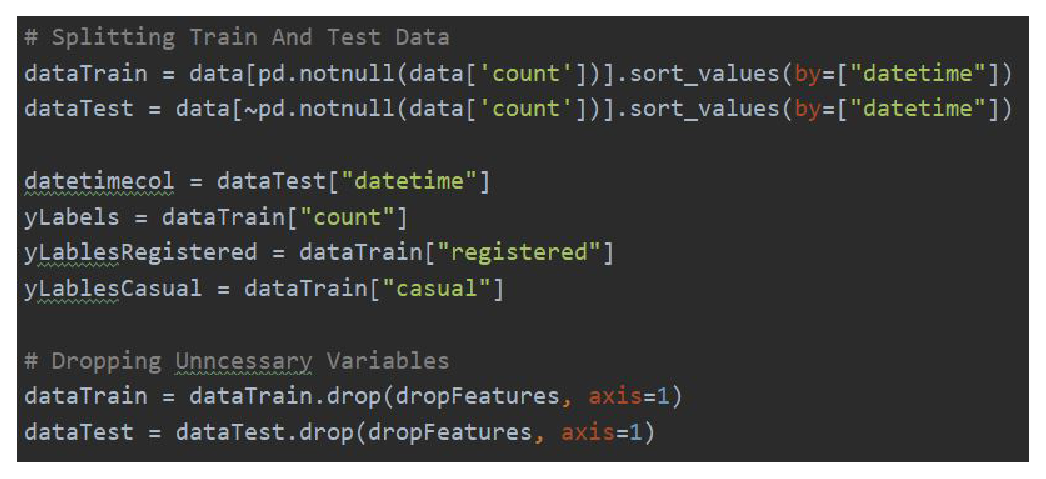
\includegraphics[scale=0.5]{./figure1/3.eps}
		\caption{Word frequency statistics of entire dataset}
	\end{figure}
\end{slide}
%%
%%==========================================================================================	

%%==========================================================================================
%%
\begin{slide}{}
	Count the number of ‘ingredients’ per cuisine. There are twenty cuisine in the train data, just show the 'Greek' word frequency statistics. Just Visualize the 25 most commonly used ingredients.
	\begin{figure}[htbp]
		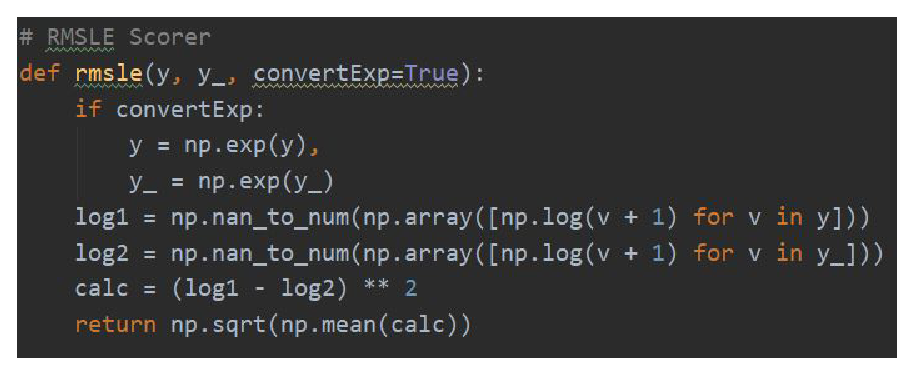
\includegraphics[scale=0.45]{./figure1/4.eps}
		\caption{Greek word frequency statistics}
	\end{figure}
\end{slide}
%%
%%==========================================================================================	

%%==========================================================================================
%%
\begin{slide}{String Preprocess}
	1:Use the WordNetLemmatizer().lemmatize() method to restore the part of speech\\
	2:remove the useless suffix of the word\\
	3:remove the non-letter symbols\\
	4:change the uppercase letters to lowercase
	\begin{figure}[htbp]
		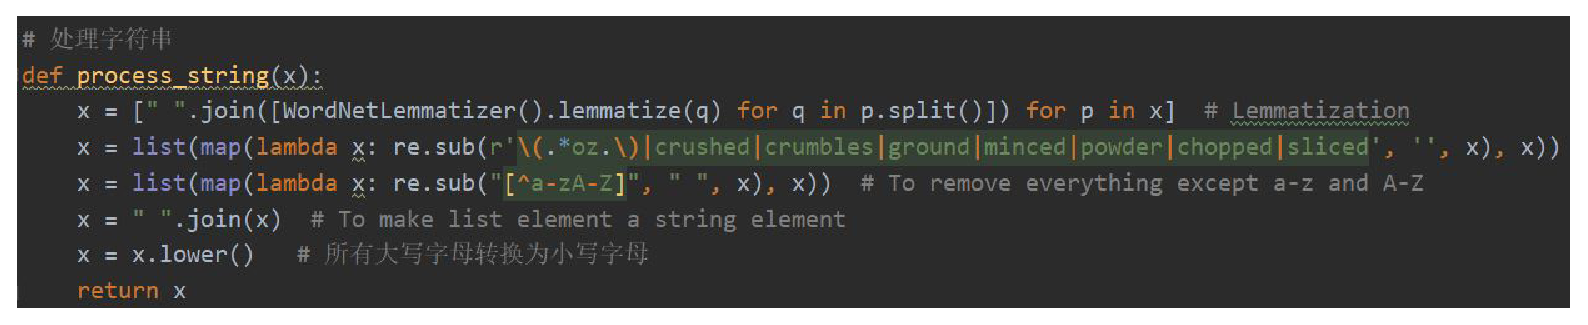
\includegraphics[scale=0.75]{./figure1/5.eps}
		\caption{String preprocess}
	\end{figure}
\end{slide}
%%
%%==========================================================================================


\section{Feature Engineering}
%%==========================================================================================
%%
\begin{slide}{Count Vectorizer}
	Convert a document into a vector by counting to complete feature extraction, which get a word frequency matrix.
	\begin{figure}[htbp]
		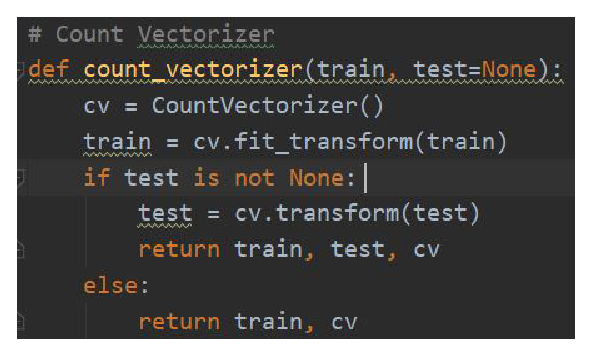
\includegraphics[scale=1.]{./figure1/6.eps}
		\caption{code of count vectorizer}
	\end{figure}
\end{slide}
%%
%%==========================================================================================	
%%==========================================================================================
%%
\begin{slide}{TFiDF Vectorizer}
	Input the word frequency matrix to get the TF-IDF weight matrix.
	\begin{figure}[htbp]
		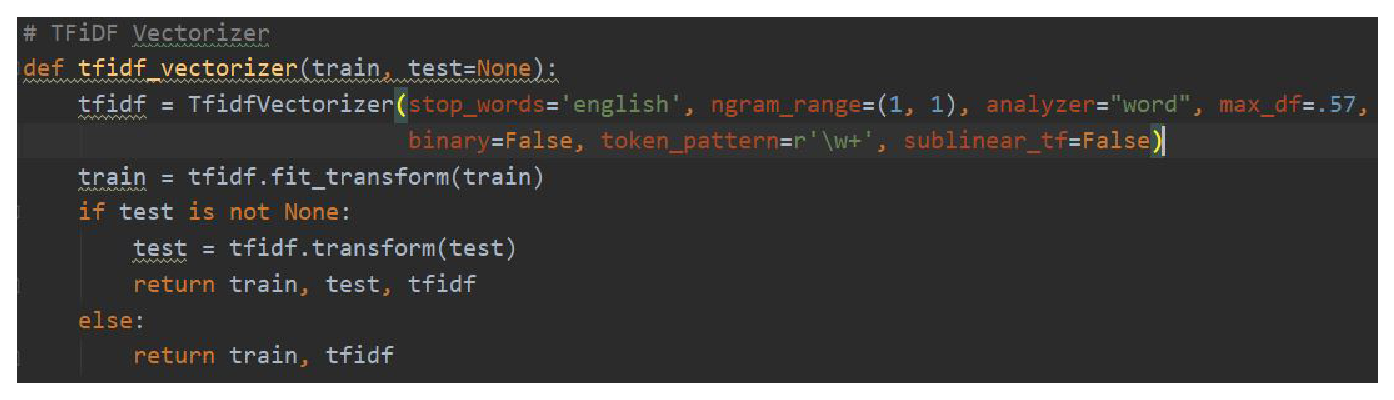
\includegraphics[scale=0.8]{./figure1/7.eps}
		\caption{code of TFiDF vectorizer}
	\end{figure}
\end{slide}
%%
%%==========================================================================================

%%==========================================================================================
\begin{slide}[toc=,bm=]{Cluster as Parameter}
	There are 20 different types of cuisine to classify. Certain groups of cuisine may have much more similarity than others. So we use the clustering information as part of the feature.\\
	
	The "cuisine\_df" is also used to generate the weight matrix through the TFiDF Vectorizer. Use PCA to reduce dimensionality.\\
	
	Predict clusters in the test data, encoded as Onehot vectors.\\
	
	Combine the TFIDF vector and the cluster vector as a feature vector.
\end{slide}

\section{Model And Conclusion}

\begin{slide}[toc=,bm=]{Model And Conclusion}
	I have choose the SVC as classification model.
	\begin{figure}[htbp]
	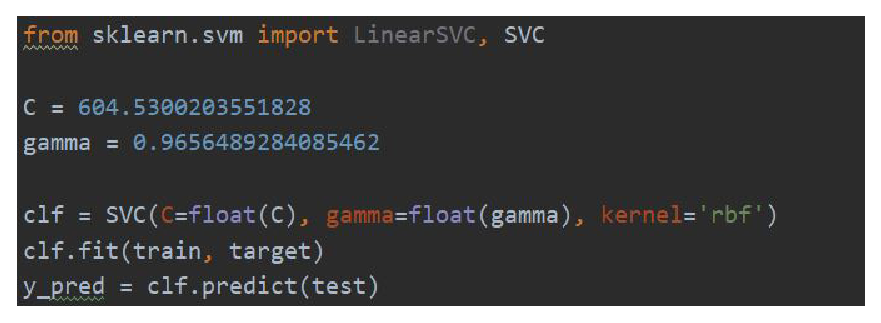
\includegraphics[scale=0.7]{./figure1/8.eps}
	\caption{SVC}
	\end{figure}
	The percentage of the number of correctly classified cuisines in the total number is used as the accuracy rate.\\
	My accuracy rate is 81.06\%
	
\end{slide}


%%
%%==========================================================================================


%%==========================================================================================
% TODO: Contact Page
\begin{wideslide}[toc=,bm=]{Contact Information}
\centering
\vspace{\stretch{1}}
\twocolumn[
lcolwidth=0.35\linewidth,
rcolwidth=0.65\linewidth
]
{
% \centerline{
\includegraphics[scale=.2]{tulip-logo.eps}}
}
{
\vspace{\stretch{1}}
Bing Liu\\
College of Computer Science and Technology\\
Jilin University, China
\begin{description}
 \item[\textcolor{orange}{\faEnvelope}] \href{mailto:bliu@tulip.academy}
 {\textsc{\footnotesize{bliu@tulip.academy}}}

 \item[\textcolor{orange}{\faHome}] \href{http://www.tulip.org.au}
 {\textsc{\footnotesize{Team for Universal Learning and Intelligent Processing}}}
\end{description}
}
\vspace{\stretch{1}}
\end{wideslide}

\end{document}

\endinput
